\documentclass[11pt]{article}
\usepackage[margin=1in]{geometry}
\usepackage{amsmath,amssymb}
\usepackage{graphicx}
\usepackage{enumitem}
\setlist[enumerate]{itemsep=0.8em}

\begin{document}

\section*{Regional 2019 -- ICTM Division AA Precalculus}
\begin{enumerate}[label=\textbf{\arabic*.}]
\item Let $k$ be the smallest positive solution for $x$ of $\sin x=0.6$, where $x$ is measured in degrees. Let $w$ be the smallest positive solution for $y$ of $\sin y=0.6$, where $y$ is measured in radians. Determine the product $kw$. Express your answer as a decimal rounded to four significant digits.\par\textit{Solution: }$23.73$.

\item The minimum value of $f(x)=A\sin(2x+\pi)+3$, where $A>0$, is $-7$. Determine the value of $A$.\par\textit{Solution: }$10$.

\item $\tan\theta=-\dfrac{7}{4}$ and $\dfrac{\pi}{2}<\theta<\dfrac{3\pi}{2}$. Then $\sin\theta=\dfrac{k\sqrt{w}}{p}$ in reduced form, with $k,w,p$ integers and $p>0$. Determine the sum $k+w+p$.\par\textit{Solution: }$137$.

\item Given the parametric function $x=4t+5$, $y=5t-1$, determine the slope of the line perpendicular to its graph when $t=-2$.\par\textit{Solution: }$-\dfrac{4}{5}$.

\item For all permissible values of $\theta$,
\[
\frac{10\sin^4\theta-17\sin^2\theta+6}{18-15\sin^2\theta}=k\cos(2\theta).
\]
Determine the value of $k$. Express your answer as an integer or as a common or improper fraction.\par\textit{Solution: }$\dfrac{1}{3}$.

\item In quadrilateral $ICTM$, $\angle ICT=90^\circ$ and $\angle CTM=115^\circ$. Also, $IC=8$, $CT=6$, and $TM=11$. Determine the numeric area of quadrilateral $ICTM$. Express your answer as a decimal rounded to the nearest thousandth.
\begin{center}
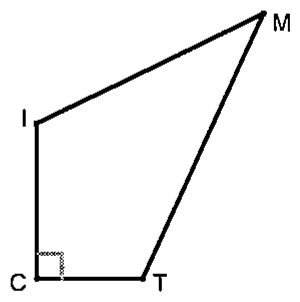
\includegraphics[width=0.5\linewidth]{diagrams/regional_2019_q06.png}
\end{center}
\par\textit{Solution: }$72.503$.

\item $f(x)=\dfrac{ax^2-11x+5}{4-11x+6x^2}$ has a horizontal asymptote at $f(x)=\dfrac{1}{3}$. Also, $b$ represents the number of distinct vertical asymptotes for the graph of $f(x)$, and $c$ represents the greatest number that is not an element of the range of $f(x)$. Determine the value of $f(b)+c$. Express your answer as an integer or as a common or improper fraction.\par\textit{Solution: }$\dfrac{29}{5}$.

\item Three integers $k,w,p$ with $k<w<p$ form a geometric sequence. The sum of these three numbers is $21$, and the sum of their reciprocals is $\dfrac{7}{12}$. Determine the three numbers. Express your answer as the ordered triple $(k,w,p)$.\par\textit{Solution: }$(3,6,12)$.

\item Andrew and Brent take turns rolling two fair standard dice until one of two things happens: Andrew gets a sum of $6$ or Brent gets a sum of $5$. Determine the probability that Brent wins when Brent goes first. Express your answer as an integer or as a common or improper fraction.\par\textit{Solution: }$\dfrac{9}{19}$.

\item The period of the graph of $y=4\sin x\cos x(\cos^2x-\sin^2x)$ can be expressed as $k\pi$. Determine the value of $k$. Express your answer as an integer or as a common or improper fraction.\par\textit{Solution: }$\dfrac{1}{2}$.

\item The equation $y=10e^{-t}\cos\left(\dfrac{t}{3}\right)$ represents a damped vibration, such as the displacement from equilibrium of the end of a stretched spring or the end of a struck tuning fork. Determine the smallest value for $t$ after which $|y|$ never exceeds ten percent of its maximum value. Express your answer as a decimal rounded to the nearest thousandth.\par\textit{Solution: }$2.049$.

\item $f(n+1)=\dfrac{3f(n)+1}{3}$ and $f(1)=5$. Determine the value of $f(2019)$. Express your answer as an integer or as a common or improper fraction.\par\textit{Solution: }$\dfrac{2033}{3}$.

\item Aune and Ella are trying to meet at the library. Aune can arrive between 3 pm and 5 pm and stay for 17 minutes. Ella can arrive between 3:30 pm and 4:30 pm and stay for 34 minutes. Determine the probability they will be at the library at the same time. Express your answer as an integer or as a common or improper fraction.\par\textit{Solution: }$\dfrac{763}{1800}$.

\item Let $a$ be a positive integer chosen at random from the interval $[1,100]$. Then let
\[
k=\frac{a}{2}+\frac{a}{3}+\frac{a}{4}+\frac{a}{5}+\frac{a}{6}+\frac{a}{7}.
\]
Determine the probability that, when $k$ is expressed as a simplified and reduced fraction, the numerator of $k$ will be prime. Express your answer as an integer or as a common or improper fraction.\par\textit{Solution: }$\dfrac{11}{100}$.

\item Three vertices of a regular octagon are used as vertices of a triangle $ABC$. The exact smallest possible ratio $k$ for
\[
\frac{\text{Area of triangle}}{\text{Area of octagon}}
\]
can be expressed as $k=\dfrac{a+b\sqrt{c}}{d}$ in reduced form, with $a,b,c,d$ integers and $d>0$. Determine the sum $a+b+c+d$.\par\textit{Solution: }$11$.

\item Determine the remainder when $(x+1)^5+(x+2)^4+(x+3)^3+(x+4)^2+(x+5)$ is divided by $(x+2)$. Express your answer as an integer or as a common or improper fraction.\par\textit{Solution: }$7$.

\item Let $i=\sqrt{-1}$ and $z=a+bi$, where $a$ and $b$ are real. When graphed in the complex plane, the roots of $z^{12}=1$ determine the vertices of a regular dodecagon. The perimeter of this regular dodecagon can be expressed as $k=m\sqrt{n}+p\sqrt{q}$, where $m,n,p,q$ are integers. Determine the sum $m+n+p+q$.\par\textit{Solution: }$8$.

\item A set of points in the $xy$-plane consists of all points satisfying the inequality $x^2+y^2<1$. The graph of this region has numeric area $Z$. A curve with equation
\[
\frac{1}{x}+\frac{1}{y}=\frac{1}{xy},\qquad xy\ne 0,
\]
separates the region into two parts. The numeric area $A$ of the larger part can be represented as $A=\dfrac{k\pi+w}{p}$ in reduced form, with $k,w,p$ integers and $p>0$. Determine the sum $k+w+p$.\par\textit{Solution: }$9$.

\item The sum of all values for $x$ in the interval $[0,2\pi]$ such that $\sqrt{3}\sin x+\cos x=\sqrt{2}$ is $k\pi$. Determine the value of $k$. Express your answer as an integer or as a common or improper fraction.\par\textit{Solution: }$\dfrac{2}{3}$.

\item The foci of an ellipse $\dfrac{x^2}{k}+\dfrac{y^2}{w}=1$ are located at $(0,\sqrt{5})$ and $(0,-\sqrt{5})$. The major axis has length $6$. Determine the sum $k+w$.\par\textit{Solution: }$13$.
\end{enumerate}

\section*{Regional 2018 -- ICTM Division AA Precalculus}
\begin{enumerate}[label=\textbf{\arabic*.}]
\item A boy travels along a path given by $r=5\sin\theta$, where $r$ is measured in feet. The distance he travels for $0\leq\theta\leq2\pi$ is $k\pi$ feet. Determine $k$.\par\textit{Solution: }$10$.

\item An owl is perched on a vertical pine tree, with its eyes 24 feet above the ground. It spots a mouse on level ground at an angle of depression of $50^\circ$. Determine the straight-line distance from the owl to the mouse, rounded to the nearest tenth of a foot.\par\textit{Solution: }$31.3$ feet.

\item $(k,w)$ is the solution to
\[
\begin{bmatrix}3&4\\2&3\end{bmatrix}
\begin{bmatrix}x\\y\end{bmatrix}
=\begin{bmatrix}3\\4\end{bmatrix}.
\]
Determine $k+w$.\par\textit{Solution: }$-1$.

\item Let
\[
k=8\left[\sum_{n=1}^{\infty}\left(\frac13\right)^n\right].
\]
Determine $k$.\par\textit{Solution: }$4$.

\item Let $W(\theta)=(\cos\theta,\sin\theta)$ be the wrapping function around the unit circle. Determine the straight-line distance between $W(\pi)$ and $W\left(\frac{\pi}{4}\right)$, rounded to the nearest thousandth.\par\textit{Solution: }$1.848$.

\item Two cruise ships leave the same port at the same time, so that the angle between their paths is $60^\circ$. The first ship travels at 16 mph and the second at 14 mph. Determine how long they have been sailing when they are 26.424 miles apart, rounded to the nearest tenth of an hour.\par\textit{Solution: }$1.7$ hours.

\item The lines $y_1=\frac14x-3$ and $y_2=5x+\frac12$ intersect. Determine the obtuse angle formed by this intersection, rounded to the nearest tenth of a degree.\par\textit{Solution: }$115.3^\circ$.

\item Let $\vec{u}=-6\vec{i}-78\vec{j}$ and $\vec{v}=117\vec{i}+k\vec{j}$, with $\vec{u}\perp\vec{v}$. Determine $k$.\par\textit{Solution: }$-9$.

\item For your answer, write the whole word \emph{Always}, \emph{Sometimes}, or \emph{Never}, whichever is correct. The graph of a certain linear function has a negative slope. Consequently, if its $x$-intercept is a negative number, then its $y$-intercept is also a negative number.\par\textit{Solution: }Always.

\item Let $\sin x=\frac13+\cos x$. Determine $\sin(2x)$.\par\textit{Solution: }$\frac89$.

\item Box A contains 3 red marbles and 6 blue marbles. Box B contains 2 red marbles and 1 blue marble. Box C contains 2 red marbles and 4 blue marbles. Two boxes are chosen at random, then one marble is chosen from each box. Determine the probability that the marbles are the same color.\par\textit{Solution: }$\frac{13}{27}$.

\item Consider the graph of $f(x)=3\sin(2x+\pi)-5$. Determine the amplitude of $f(x)$.\par\textit{Solution: }$3$.

\item Let $x$ be the degree measure of an angle such that $\tan(x)=\sqrt3$. If $0^\circ<x<720^\circ$, determine the sum of all possible distinct values of $x$.\par\textit{Solution: }$1320^\circ$.

\item $a,b,c$ are positive integers with $b<c$ such that
\[
\frac{1}{\sqrt[3]{2}-1}=a+\sqrt[3]{b}+\sqrt[3]{c}.
\]
Determine the ordered triple $(a,b,c)$.\par\textit{Solution: }$(1,2,4)$.

\item Line $a$ has slope $\frac32$ and line $b$ has slope $4$. Line $c$ bisects an angle formed by $a$ and $b$ and has positive slope. Its slope can be written as $\frac{k+w\sqrt p}{q}$, where $k,w,p,q$ are relatively prime integers and $q>0$. Determine $k+w+p+q$.\par\textit{Solution: }$243$.

\item Let $T$ be the tetrahedron bounded by the points $(0,0,0)$, $(0,0,8)$, $(0,6,0)$, and $(10,0,0)$. A unit vector $\vec{v}$ normal to the face containing $(0,0,8)$, $(0,6,0)$, and $(10,0,0)$ can be written
\[
\vec{v}=\left(\frac{x}{\sqrt{w}},\frac{y}{\sqrt{w}},\frac{z}{\sqrt{w}}\right),\qquad x>0.
\]
Determine $x+y+z+w$.\par\textit{Solution: }$816$.

\item Let $p(x)$ and $q(x)$ be quartic polynomial functions with integer coefficients such that
\[
p(1)=q(3),\quad p(2)=q(4),\quad p(3)=q(5),\quad p(4)=q(6),\quad p(5)=q(7)+k,
\]
where $k$ is a positive multiple of 23. Determine the smallest possible $k$.\par\textit{Solution: }$552$.

\item In $\triangle ABC$, with a right angle at $C$, $\frac{AC}{BA}=\frac{56}{65}$. If $\tan\angle BAC=k$, determine $k$.\par\textit{Solution: }$\frac{33}{56}$.

\item Determine
\[
k=\lim_{x\to\infty}\frac{4x+e^{-x}}{5x}.
\]
\textit{Solution: }$\frac45$.

\item A plane flying at an average speed of 420 mph at an angle of $40^\circ$ west of due north encounters a wind pushing at 20 mph at an angle of $20^\circ$ west of due south. The plane then travels at a new angle west of due north. Determine that angle, rounded to the nearest hundredth of a degree.\par\textit{Solution: }$42.42^\circ$.
\end{enumerate}

\section*{Regional 2017 -- ICTM Division AA Precalculus}
\begin{enumerate}[label=\textbf{\arabic*.}]
\item Let $k=\sin\left(\frac23\pi\right)$ and $w=\cot\left(\frac56\pi\right)$. Determine the exact product $kw$.\par\textit{Solution: }$-\frac32$.

\item $\arcsin x$ represents the inverse sine function. Determine the exact value of
\[
\arcsin\left(\cos\left(\frac76\pi\right)\right).
\]
\textit{Solution: }$-\frac{\pi}{3}$.

\item Let $f(x)=2x^2-5x-9$. Then
\[
\lim_{h\to0}\frac{f(x+h)-f(x)}{h}=kx^2+wx+p.
\]
Determine $k+w+p$.\par\textit{Solution: }$-1$.

\item A particular triangle has sides of length 20 and 17, with included angle $52^\circ$. Determine its area, rounded to the nearest thousandth.\par\textit{Solution: }$133.962$.

\item Let
\[
k=\sum_{n=0}^{\infty}18\left(\frac{17}{20}\right)^n.
\]
Determine the exact value of $k$.\par\textit{Solution: }$120$.

\item $\triangle ABC$ is a right triangle with right angle at $C$, and $AB=11$, $BD=7$, and $DA=6$. Here $D$ lies on $\overline{AC}$, as shown in the diagram. Determine $BC$, rounded to the nearest thousandth.
\begin{center}
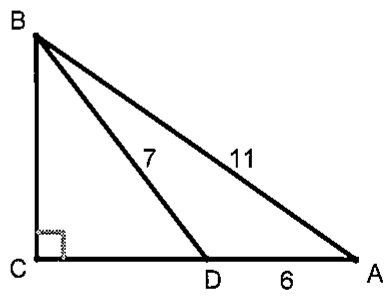
\includegraphics[width=0.5\linewidth]{diagrams/regional_2017_q06.png}
\end{center}
\par\textit{Solution: }$6.325$.

\item Matrices
\[
A=\begin{bmatrix}2&1\\5&4\end{bmatrix},\qquad B=\begin{bmatrix}7&3\\3&2\end{bmatrix}
\]
are given. Determine $\det(A\times B)$.\par\textit{Solution: }$15$.

\item A Super Ball is launched 100 feet into the air from ground level, measured vertically to the bottom of the ball. It falls back to ground level and then rebounds to $\frac34$ of its height on the previous bounce. The ball continues this pattern until it stops. Determine the total distance, in feet, that the ball traveled, measured vertically from ground level to the bottom of the ball.\par\textit{Solution: }$800$ feet.

\item The equation $(y-2)^2=5(x+3)$ in the standard coordinate system is rewritten in a coordinate system $(x',y')$ whose new origin is $(5,2)$, with axes parallel to the original $xy$-axes. The resulting equation has the form $(y')^2=k(x'+w)$, where $k,w$ are positive integers. Determine $k+w$.\par\textit{Solution: }$13$.

\item Assume the following is not a degenerate form of a conic. Identify $6x^2+5xy+2y^2+x+2y-3=0$ as a circle, ellipse, hyperbola, or parabola.\par\textit{Solution: }Ellipse.

\item Let $i=\sqrt{-1}$ and $z=1+i\sqrt3$. One square root of $z$ is $\sqrt z=a+bi$, where $a,b$ are exact real numbers in simplified radical form and $a>0$. Determine $(a,b)$.\par\textit{Solution: }$\left(\frac{\sqrt6}{2},\frac{\sqrt2}{2}\right)$.

\item Twins Jordan and Michael have the growth curves
\[
y_1=20+54\left(1-e^{-x/3}\right),\qquad y_2=21+53\left(1-e^{-x/3.1}\right),
\]
where $x$ is measured in years and $y$ in inches. Determine the sum of all years after birth at which their heights were equal, rounded to the nearest thousandth.\par\textit{Solution: }$1.738$.

\item The rectangular coordinates $(-2,-2\sqrt3)$ can be written in polar form as $(r,\theta)$, where $0\leq\theta<2\pi$ and $\theta$ is measured in radians. Determine the polar coordinates.\par\textit{Solution: }$\left(4,\frac{4\pi}{3}\right)$ (also accepted: $\left(-4,\frac{\pi}{3}\right)$).

\item In $\triangle ABC$, $\angle BAC=74^\circ$ and $AC=100$. The length of $\overline{BC}$ is an integer and is shorter than $\overline{AC}$. Determine the sum of all possible integer lengths for $\overline{BC}$.\par\textit{Solution: }$294$.

\item Today is Aune's fifteenth birthday. Her parents measure her height to be 62.5 inches; on her fourteenth birthday it was 61.0 inches. Her height has been increasing geometrically for the past five years. Determine her height, in inches, on her tenth birthday, rounded to the nearest quarter inch.\par\textit{Solution: }$55.25$ inches.

\item Let $f(x)=3+4\cos(x+\pi)$, with $x$ measured in radians. Let $k$ be the amplitude and $w$ the $y$-intercept of the graph of $f(x)$. Determine $k+w$.\par\textit{Solution: }$3$.

\item In $\triangle ABC$, $D$ lies on $\overline{AC}$ such that $\overline{BD}$ bisects $\angle ABC$. Given $AB=18$, $BC=12$, and $DC=7$, determine the smallest angle of $\triangle ABC$, in degrees, rounded to the nearest thousandth.\par\textit{Solution: }$39.482^\circ$.

\item Let $\sin\theta=-\frac12$, where $0\leq\theta<2\pi$ and $\theta$ is measured in radians. The sum of all possible values of $\theta$ is $k\pi$. Determine $k$.\par\textit{Solution: }$3$.

\item When $2\sin(2x)\cos x-4\cos^2x=\sin x-1$ is solved over $0\leq x\leq2\pi$, the sum of the solutions is $k\pi$. Determine $k$.\par\textit{Solution: }$\frac92$.

\item The directrix of a parabola with vertex $(-3,2)$ that passes through $(9,-16)$ and opens down is either $x=k$ or $y=w$. Determine its directrix.\par\textit{Solution: }$y=4$.
\end{enumerate}

\section*{Regional 2016 -- ICTM Division AA Precalculus}
\begin{enumerate}[label=\textbf{\arabic*.}]
\item Determine the value of the indicated vector inner (dot) product $(-5,3)\cdot(6,8)$.\par\textit{Solution: }$-6$.

\item Determine the value of
\[
\lim_{x\to0}\frac{5x^3+3x^2-7x+3}{2x-3}.
\]
\textit{Solution: }$-1$.

\item Let $\tan\theta=\frac12$, with $\theta$ in quadrant I. Write $\cos\theta+\cot\theta=\frac{k+w\sqrt{p}}{q}$ in simplified, reduced radical form, where $k,w,p,q$ are integers. Determine $k+w+p+q$.\par\textit{Solution: }$22$.

\item Determine the value of the sum
\[
\sum_{k=2}^{5}(2^k-1).
\]
\textit{Solution: }$56$.

\item A sine curve has a maximum value of $3$ at $x=\frac43\pi$, and a minimum value of $-3$ at $x=\frac{10}{3}\pi$, with exactly one zero between these $x$-values. Find the standard equation $y=A\sin[B(x-C\pi)]+D$ with $A>0$ as small as possible. Give $A+B+C+D$ as a reduced fraction.\par\textit{Solution: }$\frac{23}{6}$.

\item Let $f(x)=x^3+\frac32$, $g(x)=2x\sqrt{x}$, and $h(x)=\sin^2x$. Determine $f(g(h(\frac{\pi}{6})))$, as a reduced fraction.\par\textit{Solution: }$\frac{97}{64}$.

\item Let $f(x)=(x-a)(x-b)^2(x+c)$, where $0<a<b<c$. Solve $f(x)<0$, using interval notation.\par\textit{Solution: }$(-c,a)$.

\item In a geometric sequence, the last term is $1458$, the common ratio is $-3$, and the sum of the terms is $1094$. Determine the second term.\par\textit{Solution: }$-6$.

\item Let $a,b,c,d$ be positive real numbers with $a+b+c+d=10$, $c=d$, and $a^2+b^2+c^2+d^2=30$. Write the largest possible value of $c$ as $\frac{k+\sqrt w}{f}$ in reduced radical form, where $k,w,f$ are positive integers. Determine $k+w+f$.\par\textit{Solution: }$12$.

\item Determine the area of a triangle with sides $20$ and $16$, whose included angle measures $150^\circ$.\par\textit{Solution: }$80$.

\item In $\triangle ABC$, $2\sin A+3\cos B=4$ and $3\sin B+2\cos A=3$. Determine the degree measure of $\angle C$.\par\textit{Solution: }$90^\circ$.

\item The points $(1,3,-1)$, $(-2,1,5)$, and $(3,2,6)$ lie in a plane with equation $Ax+By+Cz+D=0$, where $A,B,C,D$ are relatively prime integers and $A>0$. Determine $A+B+C+D$.\par\textit{Solution: }$52$.

\item A parabola has equation $2x^2+12x=3y$. Its directrix is $x=k$ or $y=w$, as appropriate. Determine the directrix as an exact decimal.\par\textit{Solution: }$y=-6.375$.

\item $\sqrt3+\sqrt5$ is a zero of a fourth-degree polynomial with integer coefficients and leading coefficient $1$, written in decreasing powers of $x$. Determine the constant term.\par\textit{Solution: }$4$.

\item Determine the number of distinct arrangements of the letters in \emph{MATHEMATICS}.\par\textit{Solution: }$4{,}989{,}600$.

\item The roots of $x^3+ax^2+bx-105=0$ are each two more than the roots of $x^3-dx^2+ex-f=0$, where $a,b,d,e,f$ are real constants. Determine $4d+2e+f$.\par\textit{Solution: }$97$.

\item For all real $\theta$ such that $\cos\theta+\sin\theta\ne0$,
\[
\frac{\cos^3\theta+\sin^3\theta}{\cos\theta+\sin\theta}=k-w\sin(2\theta).
\]
Determine $7k+28w$.\par\textit{Solution: }$21$.

\item Let $t_1=77$ and
\[
t_{n+1}=\frac{1-24t_n}{24-3t_n},\qquad n\ge1.
\]
Determine $t_{2016}$, as a reduced fraction.\par\textit{Solution: }$\frac{1847}{207}$.

\item Determine the number of intersection points of $y=1-\frac{x}{4}$ and $y=\frac{\sin x}{x}$, where $x$ is measured in radians.\par\textit{Solution: }$2$.

\item In the diagram, $A=(0,0)$, $B=(26,0)$, $C=(x,y)$, $AC=51$, and $BC=55$. Point $P$ is inside $\triangle ABC$, and $[PAB]:[PAC]:[PBC]=1:2:3$, where brackets denote area. Determine the ordered pair for $P$, with reduced fractional coordinates.
\begin{center}
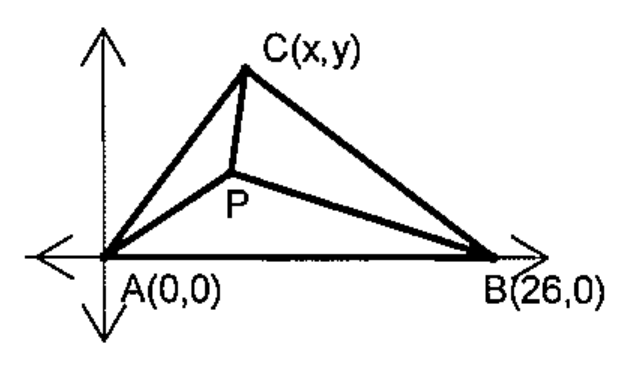
\includegraphics[width=0.5\linewidth]{diagrams/regional_2016_q20.png}
\end{center}
\par\textit{Solution: }$\left(\frac{739}{78},\frac{110}{13}\right)$.
\end{enumerate}

\section*{Regional 2015 -- ICTM Division AA Precalculus}
\begin{enumerate}[label=\textbf{\arabic*.}]
\item Points $P=(-3,4)$ and $Q=(-5,2)$ are given. Determine the exact magnitude of vector $\overrightarrow{PQ}$.\par\textit{Solution: }$2\sqrt2$.

\item $f\circ g(x)=f(g(x))$. If $f(x)=5x+6$ and $g(x)=3x-1$, then $f\circ g(x)=kx+w$. Determine $(k,w)$.\par\textit{Solution: }$(15,1)$.

\item Determine all complex roots of $x^2+40=-9$.\par\textit{Solution: }$7i,-7i$.

\item Real numbers $x$ and $y$ satisfy $x^2+3xy+y^2=60$. Determine the maximum possible value of $xy$.\par\textit{Solution: }$12$.

\item The largest real $x$ such that $\sin(3x)+\sin x=0$ on $[0,2\pi)$ is $x=k\pi$. Determine $k$, as a reduced fraction.\par\textit{Solution: }$\frac32$.

\item Consider $y=\frac12\cos(8\pi x-4)+12$. Let $k$ be its amplitude and $w$ its period. Determine $kw$, as a reduced fraction.\par\textit{Solution: }$\frac18$.

\item A sequence satisfies $F_{n+1}=F_n+F_{n-1}$, $F_4=7$, and $F_7=29$. Determine $F_{10}$.\par\textit{Solution: }$123$.

\item Solve for all $x$ such that $\log_{100}(x+2)=\log x$.\par\textit{Solution: }$2$.

\item In vector notation, $\vec v=\langle a,b\rangle=a\vec i+b\vec j$. Determine the angle between $\vec u=\langle2,3\rangle$ and $\vec v=\langle-2,5\rangle$, in degrees rounded to the nearest hundredth.\par\textit{Solution: }$55.49^\circ$.

\item The probability that a man will be alive 25 years from now is $\frac37$; independently, the probability that his wife will be alive then is $\frac45$. Determine the probability that at least one of them will be alive, as a reduced fraction.\par\textit{Solution: }$\frac{31}{35}$.

\item In the diagram, $A,B,C$ lie on a circle centered at $O$, with radius $8$; $C$ lies on the major arc $AB$, and $AB=6$. Determine $\angle C$, in degrees rounded to the nearest hundredth.
\begin{center}
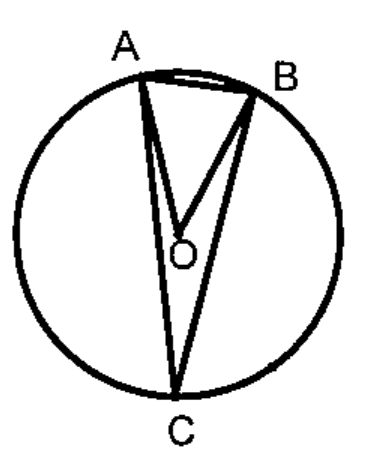
\includegraphics[width=0.5\linewidth]{diagrams/regional_2015_q11.png}
\end{center}
\par\textit{Solution: }$22.02^\circ$.

\item If $x>5$, determine the largest value of $k$ such that $\log(x)-k=\log(x-5)+3$ has no real solutions.\par\textit{Solution: }$-3$.

\item
\[
\frac{4x^4+2x^3+5x^2+15}{x+5}=Q(x)+\frac{k}{x+5}.
\]
Determine $k$.\par\textit{Solution: }$2390$.

\item Let $\angle A$ and $\angle B$ be first-quadrant angles with $\sin A=\frac47$ and $\cos B=\frac57$. In reduced, simplified radical form, write
\[
\tan(A+B)=\frac{k\sqrt p+w\sqrt q}{f},
\]
where $k,w,p,q,f$ are integers. Determine $k+w+p+q+f$.\par\textit{Solution: }$62$.

\item Evie and Xavier are playing a game rolling a fair standard six-sided die. Evie wins if she rolls a 6 before Xavier rolls an odd number. If Evie rolls first, determine the probability Evie wins the game. Express your answer as a common fraction reduced to lowest terms.\par\textit{Solution: }$\frac27$.

\item Henrik measured the angle of inclination from the ground to the top of a vertical pole along a line on level ground and found the angle to be $50^\circ$. He walked 10 feet farther from the pole along the same line and measured the angle of inclination from ground level to the top of the pole to be $40^\circ$. If he walked along that same line to a point 10 feet from the base of the pole, the angle of inclination from ground level to the top of the pole is $k^\circ$. Determine $k$. Express your answer as a decimal rounded to the nearest hundredth of a degree.\par\textit{Solution: }$70.57^\circ$.

\item Determine the point on $y=\sqrt{2x-5}$ closest to $(5,0)$, with exact coordinates.\par\textit{Solution: }$(4,\sqrt3)$.

\item When written as an integer, $2015!$ has $k$ trailing zeros. Determine $k$.\par\textit{Solution: }$502$.

\item Let $\sec\theta=\frac{20}{15}$. Determine the least possible exact value of $\sin\theta$.\par\textit{Solution: }$-\frac{\sqrt7}{4}$.

\item In the diagram, $D$ lies on $\overline{AB}$ and $\overline{CD}$ bisects $\angle ACB$; the two angles at $C$ are $\theta$, with $\cos\theta=\frac14$. The side labels are $a=BC$ and $b=CA$, and $\frac1a+\frac1b=\frac1{20}$. Determine the exact length $CD$.
\begin{center}
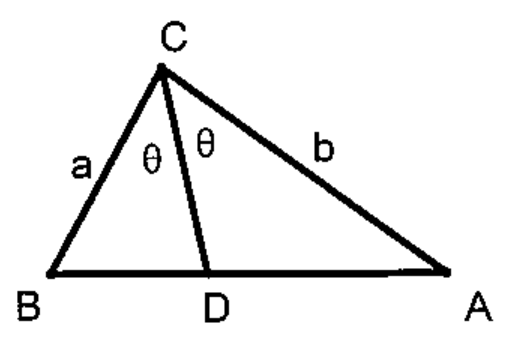
\includegraphics[width=0.5\linewidth]{diagrams/regional_2015_q20.png}
\end{center}
\par\textit{Solution: }$10$.
\end{enumerate}

\section*{Regional 2014 -- ICTM Division AA Precalculus}
\begin{enumerate}[label=\textbf{\arabic*.}]
\item One solution of $x^2+bx+c=0$, where $b,c$ are integers, is $x=1+\sqrt2$. Determine $b+c$.\par\textit{Solution: }$-3$.

\item Let $i=\sqrt{-1}$. Solve for $b$:
\[
1-\frac{b}{4+i\sqrt3}+\frac{b}{4-i\sqrt3}=0.
\]
\textit{Solution: }$\frac{19i\sqrt3}{6}$.

\item The graph of $4x^2-y^2-8x+2y=1$ is rotated $90^\circ$ clockwise about the origin. Determine the center of the new conic, as an ordered pair.\par\textit{Solution: }$(1,-1)$.

\item How many of the following polar points coincide with $(5,\frac{\pi}{6})$?
\[
\text{I. }(-5,\tfrac{7\pi}{6}),\quad\text{II. }(5,\tfrac{5\pi}{6}),\quad\text{III. }(5,\tfrac{13\pi}{6}),\quad\text{IV. }(5,\tfrac{11\pi}{6}),\quad\text{V. }(-5,-\tfrac{\pi}{6}).
\]
\textit{Solution: }$2$.

\item Find the value(s) of $x$ for which $4+3\sqrt{7-x}=x+7$.\par\textit{Solution: }$3$.

\item Simplify
\[
\cos^6x+3(\cos^4x)(\sin^2x)+3(\cos^2x)(\sin^4x)+\sin^6x.
\]
\textit{Solution: }$1$.

\item Let $P(x)$ be a monic third-degree polynomial with integer coefficients, and suppose $P(x)=0$ has at least one integer root. If $P(6)=-11$, $P(4)=3$, and $P(-4)=-341$, determine $P(10)$.\par\textit{Solution: }$177$.

\item A bag contains red and blue marbles. When two marbles are drawn, the probability of drawing two red marbles equals the probability of drawing two blue marbles. The probability of drawing one marble of each color is $\frac47$. Find the least possible number of marbles in the bag.\par\textit{Solution: }$8$.

\item The distance between $y=\frac34x+b$ and $3x-4y=7$ is $2$. If $b>0$, determine $b$.\par\textit{Solution: }$\frac34$.

\item If $i=\sqrt{-1}$, determine the sum of an infinite geometric series with first term $2-i$ and common ratio $\frac12i$.\par\textit{Solution: }$2$.

\item Determine the coefficient of $x^2y^2z^2$ in $(1+x)^5(1+y)^4(1+z)^3$.\par\textit{Solution: }$180$.

\item The solutions of $2(\ln x)^2=\ln(x^5)+3$ are of the form $e^a$. Determine the sum of all possible values of $a$, as a reduced fraction.\par\textit{Solution: }$\frac52$.

\item Given $f(4x+3)=8x-1$ and $f^{-1}(x)=ax+b$, determine $a+b$.\par\textit{Solution: }$4$.

\item Let
\[
u=2\sin x+\frac{\cos^2x}{2\sin x+\frac{\cos^2x}{2\sin x+\cdots}},
\]
where $0<\cos x<\sin x$ and $\cos x=\frac13$. Determine $u$, as a single reduced fractional expression.\par\textit{Solution: }$\frac{3+2\sqrt2}{3}$.

\item Find the number of distinct real values of $x$ for which the matrix
\[
\begin{bmatrix}x-2&x+5\\2x&x-3\end{bmatrix}
\]
does not have an inverse.\par\textit{Solution: }$2$.

\item The probability David wins exactly two games out of four equals the probability that he wins exactly three out of four. Assume game outcomes do not affect the probabilities in other games and that both players have a nonzero probability of winning. Find the probability that Jim wins any given game, as a reduced fraction.\par\textit{Solution: }$\frac25$.

\item A parabola is described parametrically by $x=2+t$, $y=1-t^2$. Find the exact distance between its vertex and its $y$-intercept.\par\textit{Solution: }$2\sqrt5$.

\item Determine the exact sum of all $\theta$ with $0\leq\theta<2\pi$ for which $\cos^2\theta=\frac35$.\par\textit{Solution: }$4\pi$.

\item The function $y=f(x)$ has period $3$. If $f(6)=4$, $f(8)=2$, and $f(10)=9$, find $2f(1)+3f(2)+4f(3)$.\par\textit{Solution: }$40$.

\item In a triangle with side lengths $a,b,c$, $(a+b+c)(a+b-c)=3ab$. Find $\sec C$, where $C$ is the angle opposite side $c$.\par\textit{Solution: }$2$.
\end{enumerate}

\section*{Regional 2013 -- ICTM Division AA Precalculus}
\begin{enumerate}[label=\textbf{\arabic*.}]
\item Given the relation $\{(2,3),(4,k),(4,2),(5,1)\}$, the product of all distinct numbers in its range is 60. Find $k$.\par\textit{Solution: }$10$.

\item Let $i=\sqrt{-1}$. Let $k$ and $w$ be positive integers with $k<w$. If $(3i)(ki)(wi)=-12i$, find $k$.\par\textit{Solution: }$1$.

\item The vector $(5.1,3.4)$ is perpendicular to $(-6.5,k)$. Find $k$ as an exact decimal.\par\textit{Solution: }$9.75$.

\item The sum of an infinite geometric series of real terms whose first term is $k$ is $\frac{2k}{k+1}$. If $k>0$ and the second term is $k^2$, find $k$ as a reduced common fraction.\par\textit{Solution: }$\frac13$.

\item Find the length of the minor axis of the conic section
\[
5x^2-10x+9y^2-72y+104=0.
\]
\textit{Solution: }$2\sqrt5$.

\item Let $i=\sqrt{-1}$, and let $k$ and $w$ be real numbers. If $(k+wi)(9-2i)=x+7i$ is solved for $x$, then $x=74-14i$. Find $k+w$.\par\textit{Solution: }$9$.

\item Bob, Christie, and Judy repeatedly take turns tossing a fair, standard cubical die. Bob begins, Christie always follows Bob, and Judy always follows Christie. Find the probability that Christie is the first to toss a die whose uppermost face displays an odd number of spots. Give a reduced common fraction.\par\textit{Solution: }$\frac27$.

\item Let $f$ be a real-valued function. If
\[
f(x)=\frac{\log(x-2)}{x^2-40}+\sqrt{8\sqrt3-x},
\]
its domain is $(k,a\sqrt b)\cup(c\sqrt d,g\sqrt h]$, where $k,a,b,c,d,g,h$ are positive integers. Find $3k+2a+b+c+d+7g+h$.\par\textit{Solution: }$91$.

\item In the diagram, $A,B,C$ lie on $\overline{FE}$, $\overline{FD}$, and $\overline{ED}$, respectively. If $EA=10$, $AF=5$, $BF=12$, $BD=22$, $CD=16$, and $CE=19$, find the area of $\triangle ABC$ as a reduced improper fraction.
\begin{center}
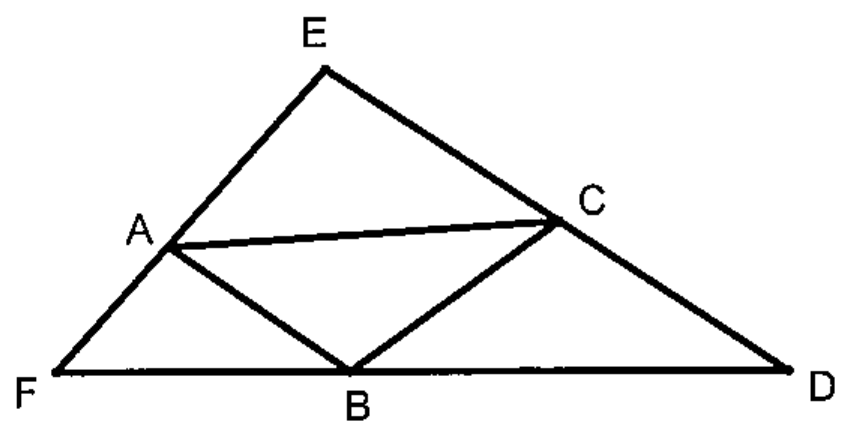
\includegraphics[width=0.5\linewidth]{diagrams/regional_2013_q09.png}
\end{center}
\par\textit{Solution: }$\frac{4812}{85}$.

\item Find the degree of the polynomial
\[
3x(x^3+5)+6\bigl(x^2(x-7)^3\bigr)^2+34x-9.
\]
\textit{Solution: }$10$.

\item There are 12 teams in a league. Each team must play every other team exactly 10 times in one season. Find the number of games played during the season.\par\textit{Solution: }$660$.

\item Find the sum of all distinct positive values of $y$ satisfying
\[
\begin{cases}
\log_9 x=\log_3 y,\\
x^2-5y^2=-6.
\end{cases}
\]
\textit{Solution: }$\sqrt2+\sqrt3$.

\item An arithmetic sequence has first term 8 and thirteenth term $-28$. Find the sum of its other eleven terms.\par\textit{Solution: }$-110$.

\item In the diagram, $AB=50$ and $BC=40$. If
\[
\frac{\sin\!\left(\tfrac12(\angle CAB-\angle CBA)\right)}{\cos\!\left(\tfrac12\angle ACB\right)}=\frac{12}{25},
\]
find the exact length $AC$.
\begin{center}
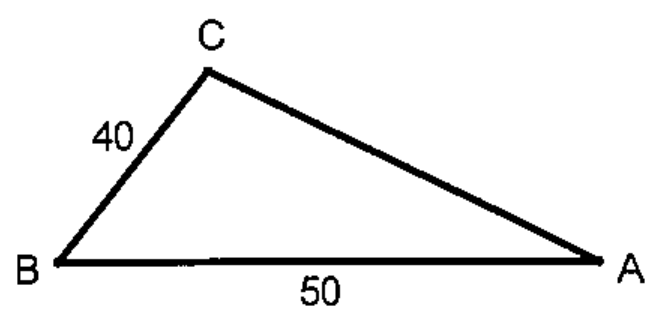
\includegraphics[width=0.5\linewidth]{diagrams/regional_2013_q14.png}
\end{center}
\par\textit{Solution: }$16$.

\item Let $i=\sqrt{-1}$, and let $k$ be real. If $7+ki^3+x=4+6i^2+3i$ is solved for $x$, then $x=-9-7i$. Find $k$.\par\textit{Solution: }$-10$.

\item Let $n$ be an integer with $0<n<6$. Two roots of
\[
x^3+nx^2-(n+1)x+k=0
\]
are additive inverses. Find the sum of all possible distinct values of $k$.\par\textit{Solution: }$-70$.

\item Katie randomly places 3 identical math books, 2 identical science books, and 2 identical English books on a shelf. Find the probability that the 3 math books are together, as a reduced common fraction.\par\textit{Solution: }$\frac17$.

\item Given $\sin A=-\frac23$ and $\pi<A<\frac{3\pi}{2}$, write $\sin(2A)$ in simplest radical form $\frac{k\sqrt w}{p}$, where $k,w,p$ are integers, $k$ and $p$ are relatively prime, and $p>0$. Find $k+w+p$.\par\textit{Solution: }$18$.

\item Let $i=\sqrt{-1}$. The factors $(x-1-2i)$, $(x-1+2i)$, and $(x-5)$ belong to the polynomial $x^3+kx^2+wx+p$, where $k,w,p$ are integers. Find $k+p$.\par\textit{Solution: }$-32$.

\item In $\triangle ABC$, let $AB=c$, $AC=b$, $BC=a$, and $\angle BAC=60^\circ$. If
\[
(a+b+c)(a+b-c)=\frac{49}{19}ab
\]
and all side lengths are integers, find the smallest possible value of $c$.\par\textit{Solution: }$21$.
\end{enumerate}

\section*{Regional 2011 -- ICTM Division AA Precalculus}
\begin{enumerate}[label=\textbf{\arabic*.}]
\item Find $\displaystyle\lim_{x\to5}2^{9-x}$.\par\textit{Solution: }$16$.

\item A sequence is defined recursively by $a_{n+1}=3a_n-5$ for all integers $n\ge1$. If $a_{10}=16$, find $a_8$.\par\textit{Solution: }$4$.

\item Let $\vec a=(3,2)$ and $\vec b=(-8,13)$. Find the ordered pair representing $3\vec a+5\vec b$.\par\textit{Solution: }$(-31,71)$.

\item Find $\displaystyle\sum_{k=2}^{5}(k^3+3.782)$ as an exact decimal.\par\textit{Solution: }$239.128$.

\item Find the tenth term of the geometric sequence whose first three terms are $\frac{1024}{5},\frac{512}{15},\frac{256}{45}$. Give a reduced common fraction.\par\textit{Solution: }$\frac{2}{98415}$.

\item The relation $f=\{(2,7),(5,3),(7,11),(19,w)\}$ is given. Find the product of all distinct real values of $w$ for which $f^{-1}$ is not a function.\par\textit{Solution: }$231$.

\item Let $k$ be a positive integer and $w$ an integer such that two roots of $x^3-17x^2+kx+w=0$ are consecutive positive integers. Find $k$ if $|k-w|$ is a maximum.\par\textit{Solution: }$26$.

\item The angle of elevation from the base of a ski lift to its summit is $35^\circ$. If a skier rides 1000 feet on the lift to the summit, find the vertical distance from the base to the summit, rounded to the nearest tenth of a foot.\par\textit{Solution: }$573.6$ feet.

\item In the diagram, $\angle CAB=30^\circ$, $AB=12$, $AC=k\sqrt3$, and $BC=w$, where $k,w$ are positive integers and $w<164$. Find the sum of all possible distinct values of $w$.
\begin{center}
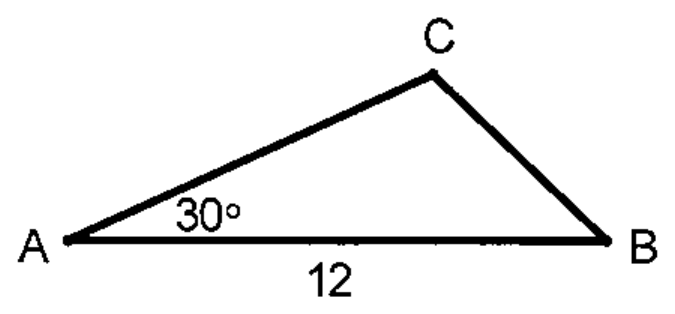
\includegraphics[width=0.5\linewidth]{diagrams/regional_2011_q09.png}
\end{center}
\par\textit{Solution: }$216$.

\item If
\[
A=\begin{bmatrix}2&3\\1&-3\end{bmatrix}\begin{bmatrix}5&4\\1&7\end{bmatrix},
\]
find $\det(A)$.\par\textit{Solution: }$-279$.

\item If $(3x-4y+z+2a)^2$ is expanded and completely simplified, find the sum of the numerical coefficients.\par\textit{Solution: }$4$.

\item Let $x$ be an integer with $0<x<150$. Find the sum of all distinct values of $x$ satisfying
\[
\tan(3x+17)^\circ<0,\qquad \sin(5x-13)^\circ>0,\qquad \cos(2x+3)^\circ<0.
\]
\textit{Solution: }$2535$.

\item The area of the ellipse
\[
\frac{(x-3)^2}{36}+\frac{(y+2)^2}{k}=1
\]
is 18 times the area of the circle $x^2+y^2=4$. Find $k$.\par\textit{Solution: }$144$.

\item In the diagram, $\triangle DEF$ is equilateral, and $A,B,C$ lie on $\overline{EF}$, $\overline{DF}$, and $\overline{DE}$, respectively. If $EA\cong FB\cong DC$, the ratio of the area of $\triangle ABC$ to the area of $\triangle DEF$ is $53:128$, $EF=256$, and $AE<AF$, find $AF$, rounded to the nearest tenth.
\begin{center}
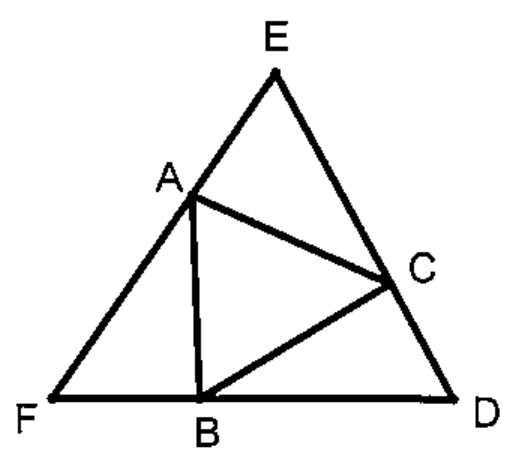
\includegraphics[width=0.5\linewidth]{diagrams/regional_2011_q14.png}
\end{center}
\par\textit{Solution: }$187.9$.

\item Given $\sin A=\frac25$ and $\frac{\pi}{2}<A<\pi$, write $\sin(2A)$ in simplest radical form $\frac{k\sqrt w}{p}$, where $k,w,p$ are integers, $k$ and $p$ are relatively prime, and $p>0$. Find $k+w+p$.\par\textit{Solution: }$42$.

\item From a group of 8 men and 7 women, a committee of 3 is selected at random. Find the probability that it consists of 2 members of one sex and 1 member of the other.\par\textit{Solution: }$\frac45$.

\item If $\sin x=\frac5{13}$ and $\cot y=-\frac34$, there are two possible values of $\tan(x-y)$. Find their sum as a reduced improper fraction.\par\textit{Solution: }$\frac{507}{112}$.

\item Let $C(n,k)=\frac{n!}{k!(n-k)!}$, where $n,k$ are positive integers. Find the sum of all distinct values of $n$ such that $97<C(n,6)<2114$.\par\textit{Solution: }$46$.

\item The graph of $g(x)=\frac{x^2-5x+6}{x-4}$ has a slant asymptote $f(x)=mx+b$. Find $m+b$.\par\textit{Solution: }$0$.

\item Let $x$ and $n$ be two-digit positive odd integers with nonzero tens digits and $n>x$. Find the largest possible $x$ for which the sum of the consecutive positive odd integers from 1 through $x$ is 99 less than the sum of the consecutive positive odd integers from $x$ through $n$.\par\textit{Solution: }$43$.
\end{enumerate}

\section*{Regional 2010 -- ICTM Division AA Precalculus}
\begin{enumerate}[label=\textbf{\arabic*.}]
\item A rectangle has a base of length 8. One of the whole numbers greater than 5.2 and less than 7.3 is selected at random for its height. Find the probability that the area is greater than 50, as a reduced common fraction.\par\textit{Solution: }$\frac12$.

\item If $f(x)=|3x-12|$, then a line of symmetry is $x=k$. Find $k$.\par\textit{Solution: }$4$.

\item Find the smallest possible positive value of $x$ for which $\cos(2x^\circ-60^\circ)=0$.\par\textit{Solution: }$75^\circ$.

\item The cubic equation with solution set $\{1,5,11\}$ can be written as $x^3+kx^2+wx+p=0$. Find $k+w+p$.\par\textit{Solution: }$-1$.

\item A geometric sequence of real numbers has first term 405 and fifth term 20480. Find its third term.\par\textit{Solution: }$2880$.

\item A circle centered at $(-6,3)$ contains the point $(2,-12)$. An arc of the circle measures $35^\circ15'$. Find the area of the sector bounded by two radii and the arc, rounded to the nearest tenth.\par\textit{Solution: }$88.9$.

\item One of the transformations necessary to produce the graph $y=2x^2+24x-1$ from $y=x^2$ is a vertical shift $k$ units downward. Find $|k|$.\par\textit{Solution: }$73$.

\item The function $g$ satisfies $g(x)+g(y)=g(x+y)+2xy-8$ for every pair of real numbers $(x,y)$. If $g(1)=22$, find $g(-11)$.\par\textit{Solution: }$-470$.

\item When $y^2+my+14$ is divided by $y-3$, the quotient is $f(y)$ and the remainder is $k$. When it is divided by $y-7$, the quotient is $g(y)$ and the remainder is $w$. If $w=2k+1$, find $m$.\par\textit{Solution: }$-16$.

\item All side lengths of a triangle are integers. The cosine of its smallest angle is $\frac{19}{21}$, and one of the sides adjacent to that angle has length 6. Find the smallest possible perimeter.\par\textit{Solution: }$16$.

\item Two letters are selected at random without replacement from $\{A,B,C,D,E,F\}$. Find the probability that $A$, $B$, or both are selected, as a reduced common fraction.\par\textit{Solution: }$\frac35$.

\item If $\ln$ denotes the natural logarithm, find $y$ such that
\[
\ln(5+4y)-\ln(3+y)=\ln(3).
\]
\textit{Solution: }$4$.

\item In $\triangle ABC$, $AB=64$, $BC=64$, and $AC=48$. The vertices $A,B,C$ are the centers of three mutually externally tangent circles, whose points of tangency are $D,E,F$. Find the perimeter of $\triangle DEF$, rounded to the nearest whole number.\par\textit{Solution: }$84$.

\item Last year, UIC tracked job placement for its high school mathematics teacher candidates, and all found teaching jobs. The arithmetic mean salary of candidates who took jobs in Chicago was \$48{,}600. The arithmetic mean for candidates who took jobs outside Chicago was \$43{,}800, and the overall mean was \$45{,}000. Find the fraction of candidates who took jobs outside Chicago, as a reduced common fraction.\par\textit{Solution: }$\frac34$.

\item A farmer wants to fence a rectangular plot of land bounded on one side by a river. He has 2200 feet of chain-link fence and will not fence the river side. Each of the two widths perpendicular to the river needs double-layer fencing. If the enclosed area is to be maximized, find the length of the field parallel to the river. Ignore the thickness of the double fencing.\par\textit{Solution: }$1100$.

\item For which two values of $x$ do the terms $x-2$, $x+1$, and $4x-8$, in that order, form a geometric progression? Find the absolute value of their difference.\par\textit{Solution: }$4$.

\item (Multiple choice.) Write A if the conditions determine a conic, B if they overdetermine a conic (that is, there is no conic meeting all the given conditions), or C if they underdetermine a conic (that is, there is more than one conic that meets all the given conditions). Ellipse with center $(0,0)$ and eccentricity $\frac23$.\par\textit{Solution: }C.

\item If $\sin(3x^\circ)=\frac12$ and $133^\circ<x<178^\circ$, find $x$.\par\textit{Solution: }$170^\circ$.

\item A hyperbola has latus rectum $24.12$, eccentricity $3.62$, center $(8.16,19.02)$, and principal axis parallel to the $y$-axis. One focus is $(x,y)$. Find the largest possible value of $y$, rounded to the nearest hundredth.\par\textit{Solution: }$22.63$.

\item Find the absolute distance from the point $(1,4,9)$ to the plane through $(5,0,4)$, $(1,7,3)$, and $(2,8,0)$, rounded to the nearest thousandth.\par\textit{Solution: }$1.028$.
\end{enumerate}

\section*{Regional 2009 -- ICTM Division AA Precalculus}
\begin{enumerate}[label=\textbf{\arabic*.}]
\item
\[
\begin{bmatrix}3&2\\4&6\end{bmatrix}
\begin{bmatrix}5\\-1\end{bmatrix}
=\begin{bmatrix}k\\w\end{bmatrix}.
\]
Find $2k+3w$.\par\textit{Solution: }$68$.

\item Given the set
\[
\left\{\log_2(16),\log_3(16),\log_4(16),\log_5(16)\right\},
\]
if one of its four members is drawn at random, find the probability that the member drawn could represent a positive integer. Express your answer as a common fraction reduced to lowest terms.\par\textit{Solution: }$\frac12$.

\item Find the ordered pair that represents the sum of the vectors $(-5,6)$ and $(17,7)$.\par\textit{Solution: }$(12,13)$.

\item Let $n$ be a positive integer. For $n\ge1$, $x_{n+2}=x_n+x_{n+1}$. If $x_1=3$ and $x_2=1$, find $x_{10}$.\par\textit{Solution: }$97$.

\item Matrix $A$ contains 23 rows and 13 columns. Matrix $B$ contains 13 rows and 92 columns. Find the number of rows in the product matrix $AB$.\par\textit{Solution: }$23$.

\item In $\triangle ABC$, the side lengths are as shown, and $\angle ABC=120^\circ$. Find the exact length of $\overline{AC}$. The diagram gives $AB=20$ and $BC=80$.
\begin{center}
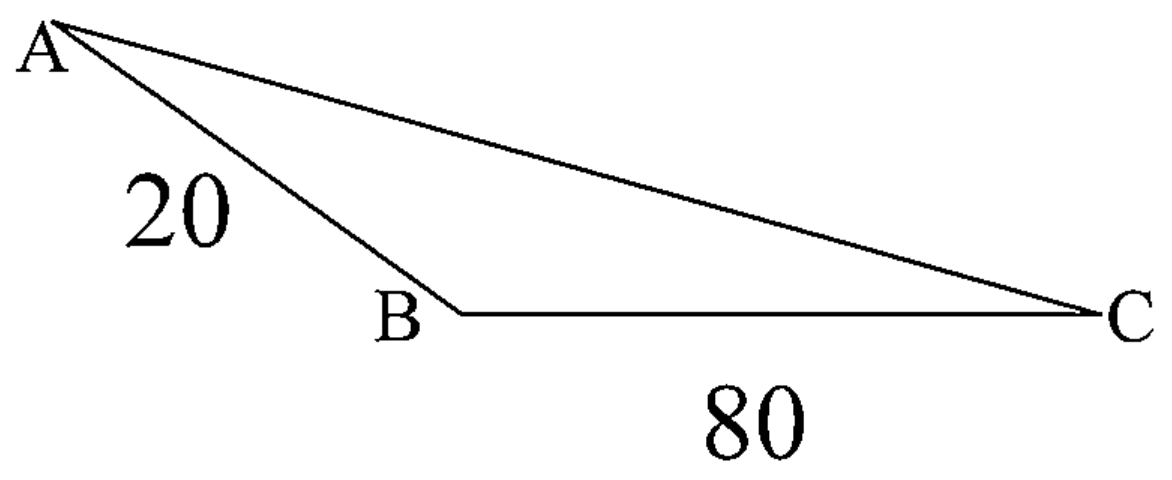
\includegraphics[width=0.5\linewidth]{diagrams/regional_2009_q06.png}
\end{center}
\par\textit{Solution: }$20\sqrt{21}$.

\item A woman is sitting in the stands behind one end zone of a football field. She observes, in the same vertical plane as her position, two players standing on their own goal lines, exactly 100 yards apart. Looking at the spots on the ground where they are standing, a player at one goal line is at an angle of depression of $15^\circ$, and a player at the other goal line is at an angle of depression of $8^\circ$. Assuming the football field is horizontal, find the number of feet in the vertical height of the woman's eye above the horizontal plane of the football field. Express your answer as a decimal rounded to the nearest hundredth of a foot.\par\textit{Solution: }$88.67$ feet.

\item If three real geometric means are inserted between 15 and $\frac{5}{27}$, find the value of the middle term. Express your answer as an improper fraction reduced to lowest terms.\par\textit{Solution: }$\frac53$.

\item In the diagram, $\triangle CAB$ is a right triangle with $\angle CAB=90^\circ$. Point $D$ is on $\overline{BC}$ such that $\overline{AD}\perp\overline{BC}$. Let the side lengths of $\triangle CAB$ opposite $\angle A,\angle B,$ and $\angle C$ be $a,b,$ and $c$, respectively. If
\[
b\sin C\left(b\cos C+c\cos B\right)=41
\]
and the length of $\overline{AD}$ is an integer, find the largest possible value of $AD$.
\begin{center}
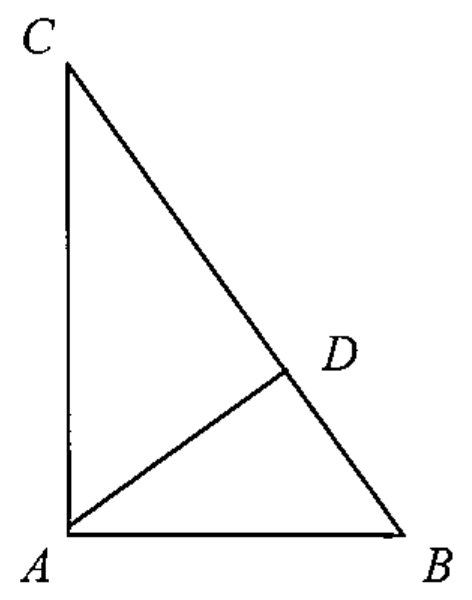
\includegraphics[width=0.5\linewidth]{diagrams/regional_2009_q09.png}
\end{center}
\par\textit{Solution: }$4$.

\item The roots of $x^3+kx^2-59x+420=0$ are 5, $-7$, and 12. Find $k$.\par\textit{Solution: }$-10$.

\item When $(2x-3)^8$ is expanded and completely simplified, find the numerical coefficient of $x^5$.\par\textit{Solution: }$-48384$.

\item The first term of an infinite geometric sequence of real terms is 225, and the fourth term is 14.4. Find the sum of the terms of this infinite geometric sequence.\par\textit{Solution: }$375$.

\item The sum of the terms of an arithmetic sequence with 13 terms and common difference 3 is 286. Find the thirteenth term of this sequence.\par\textit{Solution: }$40$.

\item Let there be $k$ objects, each of weight $w$. When these objects are weighed in pairs, the sum of the weights of all possible pairs is 770. When they are weighed in groups of four, the sum of the weights of all possible groups of four is 9240. Find $k+w$.\par\textit{Solution: }$18$.

\item Let $i=\sqrt{-1}$. Find the exact value of $\left|\sqrt6+i\sqrt8\right|$. Write your answer in simplified radical form.\par\textit{Solution: }$\sqrt{14}$.

\item Tom is a gambler. He has a pair of fair, standard cubical dice. He selects two different numbers in advance from the face numbers 1, 2, 3, 4, 5, and 6. He then rolls the pair of dice. If both numbers showing match his two selections, he wins \$108. If exactly one number showing matches one of his two selections, he neither wins nor loses. If neither number showing matches either of his two selections, he loses \$54. Find Tom's mathematical expectation each time he rolls the pair of dice. Express your answer by including the word ``lose'' or the word ``win.''\par\textit{Solution: }lose \$18.

\item Let $D$ be the point that is $\frac13$ of the way from $B$ to $A$ for equilateral triangle $\triangle ABC$. Let $P$ be a point on $\overline{BC}$ such that $AP+PD$ is the smallest possible value. If the perimeter of $\triangle ABC$ is 63, find the exact value of $AP+PD$.\par\textit{Solution: }$7\sqrt{13}$.

\item Let $i=\sqrt{-1}$ and let $k$ and $w$ represent real numbers. If $(k+wi)(4+i)=33-13i$, find the value of $k+w$.\par\textit{Solution: }$2$.

\item Find the acute angle between the normal vectors of the following two planes:
\[
3x+2y+5z+4=0\qquad\text{and}\qquad -2x-3y+6z-2=0.
\]
Round your answer to the nearest minute and then express your answer in degrees and minutes in the form $k^\circ w'$.\par\textit{Solution: }$65^\circ21'$.

\item Points $A$, $B$, $C$, and $D$ are the vertices of a rectangle. Point $E$ is in the interior of this rectangle. $AE=8$, $EC=21$. The lengths of $\overline{DE}$, $\overline{BE}$, and $\overline{BC}$ are integers. If $DE<BE$, find the largest possible value for the length of $\overline{BC}$.\par\textit{Solution: }$19$.
\end{enumerate}

\end{document}
